\documentclass[oneside, 11pt]{article}

\usepackage[T1]{fontenc}
\usepackage[utf8]{inputenc}
\usepackage[english]{babel}

\usepackage{fouriernc}
\usepackage[detect-all, binary-units, separate-uncertainty=true,
            per-mode=symbol, retain-explicit-plus, retain-unity-mantissa=false]{siunitx}

\usepackage{setspace}
\setstretch{1.2}

\setlength{\parskip}{\smallskipamount}
\setlength{\parindent}{0pt}

\usepackage[headheight=14pt]{geometry}
\geometry{marginparwidth=0.5cm, verbose, a4paper, tmargin=3cm, bmargin=3cm,
          lmargin=2cm, rmargin=2cm}

\usepackage{float}

\usepackage[fleqn]{amsmath}
\numberwithin{equation}{section}
\numberwithin{figure}{section}

\usepackage{graphicx}
\graphicspath{{images/}{../../../images/}}

\usepackage{tikz}
\usetikzlibrary{shapes}
\usetikzlibrary{plotmarks}

\newcounter{Exercise}
\setcounter{Exercise}{1}
\usepackage{xcolor}
\definecolor{shadecolor}{gray}{0.9}
\usepackage{framed}
\usepackage{caption}

\usepackage{url}


\usepackage{fancyhdr}
\pagestyle{fancy}
\fancyhf{}
\rhead{\thepage}
\renewcommand{\footrulewidth}{0pt}
\renewcommand{\headrulewidth}{0pt}

\fancypagestyle{firststyle}
{
    \fancyhf{}
    \rhead{\thepage}
    \cfoot{
\includegraphics[height=30pt]{HiSPARClogo}}
    \rfoot{
\includegraphics[height=25pt]{CCbysa}}
    \lfoot{
\includegraphics[height=30pt]{NIKHEFlogo}}
    \renewcommand{\footskip}{50pt}
    \renewcommand{\footrulewidth}{0.1pt}
    \renewcommand{\headrulewidth}{0pt}
}

\newcommand{\figref}[1]{Figuur~\ref{#1}}

\newcommand{\hisparc}{\textsmaller{HiSPARC}\xspace}
\newcommand{\kascade}{\textsmaller{KASCADE}\xspace}
\newcommand{\sapphire}{\textsmaller{SAPPHiRE}\xspace}
\newcommand{\jsparc}{\textsmaller{jSparc}\xspace}
\newcommand{\hdf}{\textsmaller{HDF5}\xspace}
\newcommand{\aires}{\textsmaller{AIRES}\xspace}
\newcommand{\csv}{\textsmaller{CSV}\xspace}
\newcommand{\python}{\textsmaller{PYTHON}\xspace}
\newcommand{\corsika}{\textsmaller{CORSIKA}\xspace}
\newcommand{\labview}{\textsmaller{LabVIEW}\xspace}
\newcommand{\daq}{\textsmaller{DAQ}\xspace}
\newcommand{\adc}{\textsmaller{ADC}\xspace}
\newcommand{\hi}{\textsc{h i}\xspace}
\newcommand{\hii}{\textsc{h ii}\xspace}
\newcommand{\mip}{\textsmaller{MIP}\xspace}
\newcommand{\hisparcii}{\textsmaller{HiSPARC II}\xspace}
\newcommand{\hisparciii}{\textsmaller{HiSPARC III}\xspace}

\DeclareSIUnit{\electronvolt}{\ensuremath{\mathrm{e\!\!\:V}}}

\DeclareSIUnit{\unitsigma}{\ensuremath{\sigma}}
\DeclareSIUnit{\mip}{\textsmaller{MIP}}
\DeclareSIUnit{\adc}{\textsmaller{ADC}}

\DeclareSIUnit{\gauss}{G}
\DeclareSIUnit{\parsec}{pc}
\DeclareSIUnit{\year}{yr}



\begin{document}

\title{Deeltjes in Airshowers}
\author{N.G. Schultheiss}
\date{}

\maketitle
\thispagestyle{firststyle}

\section{Inleiding}

Deze module volgt op de module ``Krachten in het standaardmodel''.
Deze module probeert een beeld te geven van het ontstaan van airshowers
(in de atmosfeer) uit kosmische straling (in de ruimte). De module
``Kosmische straling'' geeft inzage in de aard van kosmische straking.


\section{De eerste botsing}


\subsection{Wat botst er met elkaar?}

De kosmische straling botst boven in de atmosfeer op deeltjes in de
atmosfeer. Als vuistregel kunnen we zeggen dat een golf alleen met
een deeltje kan botsen als de golflengte kleiner is dan de diameter
van het deeltje. Langere golven stromen als het ware om het deeltje
heen. Een eerste vraag is daarom of we iets over de golflengte van
de deeltjes kunnen zeggen. Volgens De Broglie kunnen deeltjes ook
als golf worden gezien. De energie voor deeltjes is volgens Einstein:

\begin{equation}
E=mc^{2}
\end{equation}


Volgens Planck geldt:

\begin{equation}
E=h\nu=h\frac{c}{\lambda}
\end{equation}


Uitwerken geeft:
\begin{equation}
\lambda=\frac{hc}{E}=\frac{h}{mc}
\end{equation}



\paragraph*{Opdracht 1:}

\emph{Bereken je eigen golflengte en de golflengte van een H-atoom.
Waar kun je het nauwkeurigst mee meten?}

Boven in de atmosfeer worden regelmatig deeltjes met energieniveaus in
de orde van GeV \footnote{1eV is de energie die 1 elektron krijgt als
het een spanningsverschil van 1V doorloopt. Aangezien de lading van 1
elektron ongeveer $1.6*10^{-19}\mathrm{C}$ is, geldt
$1\mathrm{eV}\approx1.6*10^{-19}\mathrm{J}$.} en zelfs TeV en hoger
waargenomen.


\paragraph*{Opdracht 2:}

\emph{In de Large Hadron Collider hoopt men protonen met een energie van
7TeV te maken. Vergelijk deze golflengte met de diameter van protonen in
rust en quarks} \footnote{De grootte van een proton en een quark zijn op
internet te vinden.}\emph{. Wat is je conclusie?}


\subsection{Kan kosmische straling worden gesimuleerd in een laboratorium?}

In een laboratoriumomgeving zijn deze botsingen gecontroleerd te maken.
Een vraag die we ons kunnen stellen is, of botsingen die in de LHC
gemaakt worden, te vergelijken zijn met botsingen van kosmische straling
in de atmosfeer. Een eerste vraag is: Hoe snel gaan de protonen in
de LHC?

We kunnen de snelheid van een proton met een energie van 7TeV is op
de volgende wijze berekenen:

\begin{equation}
E=\gamma mc^{2}
\end{equation}


Waarin $\gamma=\frac{1}{\sqrt{1-\left(\frac{v}{c}\right)^{2}}}$.
Omdat de rustmassa van een proton ongeveer $\frac{938.3\mathrm{MeV}}{c^{2}}$
is, krijgen we:

\begin{equation}
7\mathrm{TeV}=\gamma*938.3\mathrm{MeV}
\end{equation}


\begin{equation}
\gamma=7.5*10^{3}=\frac{1}{\sqrt{1-\left(\frac{v}{c}\right)^{2}}}
\end{equation}


\begin{equation}
1-\left(\frac{v}{c}\right)^{2}=1.8*10^{-8}
\end{equation}


\begin{equation}
\beta=\frac{v}{c}=\sqrt{1-1.8*10^{-8}}\approx1
\end{equation}


We kunnen dus concluderen dat de protonen bijna de lichtsnelheid hebben.
In de LHC vinden duidelijk een relativistische botsingen plaats. In
de module ``Relativiteit'' hebben we gezien dat zowel energie als
impuls afhangen van de waarnemer. 

\begin{equation}
\begin{array}{c}
p_{x'}=\gamma\left(p_{x}-\beta\frac{E}{c}\right)\\
p_{y'}=p_{y}\\
p_{z'}=p_{z}\\
\frac{E'}{c}=\gamma\left(\frac{E}{c}-\beta p_{x}\right)
\end{array}
\end{equation}


Impuls en energie zijn geen invariant, de (rust)massa is overigens
wel invariant en hangt dus niet van de waarnemer af. We kunnen de
botsing van kosmische straling in de atmosfeer op verschillende manieren
waarnemen. In figuur 2.1c zien we een assenstelsel dat aan de aarde
is gekoppeld. Zoals te zien is, staat het doel van de botsing (target)
stil. Het assenstelsel is aan het ``laboratorium'' gekoppeld.

In figuur 2.1b Laten we het assenstelsel bewegen. In figuur 2.1a is
het assenstelsel gekoppeld aan het zwaartepunt van de twee botsende
deeltjes, men noemt dit massacentraal. Een massacentrale botsing heeft
het voordeel dat de som van de impulsen nul is, of $\Sigma p'=0\frac{\mathrm{eV}}{c}$.
Het accent bij $p'$ heeft overigens niet te maken met de afgeleidde
van $p$, maar wil zeggen dat dit de impuls is die door de massacentrale
waarnemer wordt waargenomen. 

\begin{figure}[H]
\noindent \begin{centering}
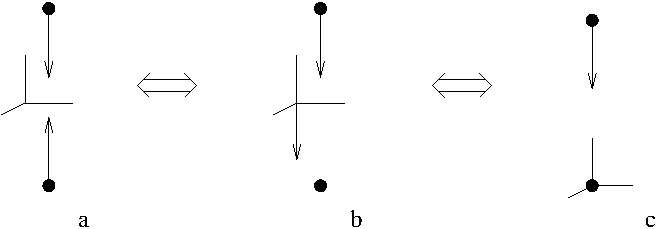
\includegraphics[scale=0.75]{assenstelsel}
\par\end{centering}

\caption{De assenstelsels van verschillende waarnemers}
\end{figure}


Voor iedere waarnemer in ieder assenstelsel geldt:

\begin{equation}
\left(\sum m_{i}^{2}\right)c^{4}
=\left(\sum E_{i}\right)^{2}+\left(\sum p_{i}\right)^{2}c^{2}
\end{equation}


Om de energie van een bewegend deeltje dat tegen een stilstaand deeltje
botst te vergelijken, kunnen we twee waarnemers gebruiken. De ene
waarnemer reist met het centrum van de botsing mee. Dit is de botsingscentrale
waarnemer. De andere waarnemer zweeft ergens in de buurt van het stilstaande
atoom waartegen gebotst wordt, dit is de laboratoriumwaarnemer.

massacentraal geldt in de LHC:

\begin{equation}
E'_{a}=E'_{b}=7\mathrm{TeV}\Longrightarrow\Sigma E'=\mathrm{14TeV}
\end{equation}


\begin{equation}
\Sigma p'=p'_{a}+p'_{b}=0\frac{\mathrm{eV}}{c}
\end{equation}


Formule (2.10) wordt:

\begin{equation}
\left(\sum m_{i}^{2}\right)c^{4}=\left(\sum E'_{i}\right)^{2}
\end{equation}


Omdat de massa volgens de botsingscentrale waarnemer en de
laboratoriumwaarnemer hetzelfde is, krijgen we nu:

\begin{equation}
\left(\sum E'_{i}\right)^{2}
=\left(\sum E_{i}\right)^{2}+\left(\sum p_{i}\right)^{2}c^{2}
\end{equation}


Nu is te zien dat de grootheden volgens de laboratoriumwaarnemer worden
geschreven zonder accent. Ten opzichte van de atmosfeer geldt, als
een kosmisch deeltje \emph{a} op een proton \emph{b} botst:

\begin{equation}
\begin{array}{c}
E_{b}=938.3\mathrm{MeV}\\
p_{b}=0\mathrm{\frac{kgm}{s}}
\end{array}
\end{equation}


Hierin is $E_{b}$ de rustmassa / energie van het proton in de atmosfeer
en $p_{b}$ de impuls. Invullen geeft:

\begin{equation}
\left(14\mathrm{TeV}\right)^{2}
=\left(E_{a}+938.3\mathrm{MeV}\right)^{2}+p_{a}^{2}c^{2}
\end{equation}


We hebben nu de variabelen $E_{a}$ en $p_{a}$ voor het kosmisch
deeltje. We kunnen kijken of er een verband tussen $E$ en $p$ bestaat.
De energie is volgens Einstein te schrijven en de impuls is te schrijven
als de waargenomen massa maal de snelheid. De waargenomen massa neemt
overigens met de lorentzconstante $\gamma$ toe als de snelheid toeneemt. 

\begin{equation}
\begin{array}{c}
E=m\gamma c^{2}\\
p=m\gamma v
\end{array}
\end{equation}


Uitwerken geeft:

\begin{equation}
p=\frac{v}{c}\frac{E}{c}
\end{equation}


De verhouding $\frac{v}{c}$ wordt over het algemeen aangeduid met
$\beta$.

\begin{equation}
p=\beta\frac{E}{c}
\end{equation}


Substitutie geeft:

\begin{equation}
\left(14\mathrm{TeV}\right)^{2}
=\left(E_{a}+938.3\mathrm{MeV}\right)^{2}+\left(\beta\frac{E_{a}}{c}\right)^{2}c^{2}
\end{equation}


Omdat de waarnemer tegen het deeltje in reist, geldt volgens formule
2.8 bij benadering $\beta\approx-1$:

\begin{equation}
\left(14\mathrm{TeV}\right)^{2}
=\left(E_{a}+938.3\mathrm{MeV}\right)^{2}-\left(\frac{E_{a}}{c}\right)^{2}c^{2}
\Longleftrightarrow
\end{equation}


\begin{equation}
\left(14\mathrm{TeV}\right)^{2}
=E_{a}^{2}+2*E_{a}*938.3\mathrm{MeV}+\left(938.3\mathrm{MeV}\right)^{2}-E_{a}^{2}
\Longleftrightarrow
\end{equation}


\begin{equation}
\left(14\mathrm{TeV}\right)^{2}
=2*E_{a}*938.3\mathrm{MeV}+\left(938.3\mathrm{MeV}\right)^{2}
\Longleftrightarrow
\end{equation}


\begin{equation}
E_{a}=\frac{\left(14\mathrm{TeV}\right)^{2}-\left(938.3\mathrm{MeV}\right)^{2}}{2*938.3\mathrm{MeV}}
=1.0*10^{17}\mathrm{eV}
\end{equation}


De protonen in de kosmische straling hebben dus vrij veel energie
$\left(E_{a}=1.0*10^{17}\mathrm{eV}\right)$. Kosmische straling met
een dergelijke energie is weliswaar zeldzaam, maar de boven een school
vindt een dergelijke botsing ongeveer 1 maal per jaar plaats.


\section{Na de eerste botsing}

Zolang we botsingen steeds massacentraal beschouwen zal $\Sigma p=0\frac{\mathrm{eV}}{c}$.
De energie kan dan helemaal worden gebruikt om deeltjes te maken.
Zoals te zien is, hebben we energie genoeg en kunnen er bijgevolg
veel verschillende soorten deeltjes gemaakt worden. De deeltjes die
we op Aarde kunnen meten, moeten stabiel genoeg zijn om de detector
op de Aarde te bereiken.

In de praktijk zijn de gemeten deeltjes in de meeste gevallen muonen.
Een tau heeft een halfwaardetijd van $2.906*10^{-13}\mathrm{s}$,
een muon heeft een halfwaardetijd van $2.197019*10^{-6}\mathrm{s}$
en een elektron ($\beta$-straling) is stabiel. Zoals we hebben gezien
bewegen deze deeltjes met snelheden tegen de lichtsnelheid. Omdat
deze ongeveer $3*10^{8}\frac{m}{s}$ is, lijkt het op het eerste gezicht
dat de helft van de muonen een afstand van maximaal 660m afleggen.
Omdat we op een hoogte van 660m best adem kunnen halen, lijkt deze
waarde wat klein.

Volgens de relativiteitstheorie gaat de tijd echter langzamer als
je met een snelheid beweegt, er geldt namelijk: $t'=\gamma\left(t-\frac{vx}{c^{2}}\right)$.
Als een deeltje tegen de lichtsnelheid beweegt, wordt $\gamma$ groot
en wordt de halfwaardetijd voor de waarnemer veel groter dan die voor
het deeltje. Bijgevolg beweegt het deeltje veel verder.

Helaas is deze tijdsvertraging voor een tau niet voldoende om bij
de detector te komen. De elektronen dragen bij aan het ioniseren van
de lucht en verdwijnen daardoor als straling. 


\paragraph*{Opdracht 3:}

\emph{Neem aan dat muonen met de halve lichtsnelheid ten op zichte
van de atmosfeer bewegen, hoever komt de helft van de muonen dan?}


\paragraph*{Opdracht 4:}

\emph{Een tweede groep muonen bewegen met 99\% van de lichtsnelheid.
Hoever komt de helft van de muonen nu?}


\paragraph*{Opdracht 5:}

\emph{Hoever komt de helft van de tau's die met 99\% van de lichtsnelheid
bewegen?}


\section{De shower}

Afhankelijk van de dichtheid van de atmosfeer en de snelheid van de
ontstane deeltjes, is er een kans dat deze deeltjes weer botsen. Bij
iedere botsing wordt een deel van de energie omgezet in deeltjes die
eventueel weer kunnen vervallen. Als we de ontstane deeltjes als functie
van de hoogte willen schetsen, ontstaat de volgende grafiek:

\begin{figure}[H]
\noindent \begin{centering}
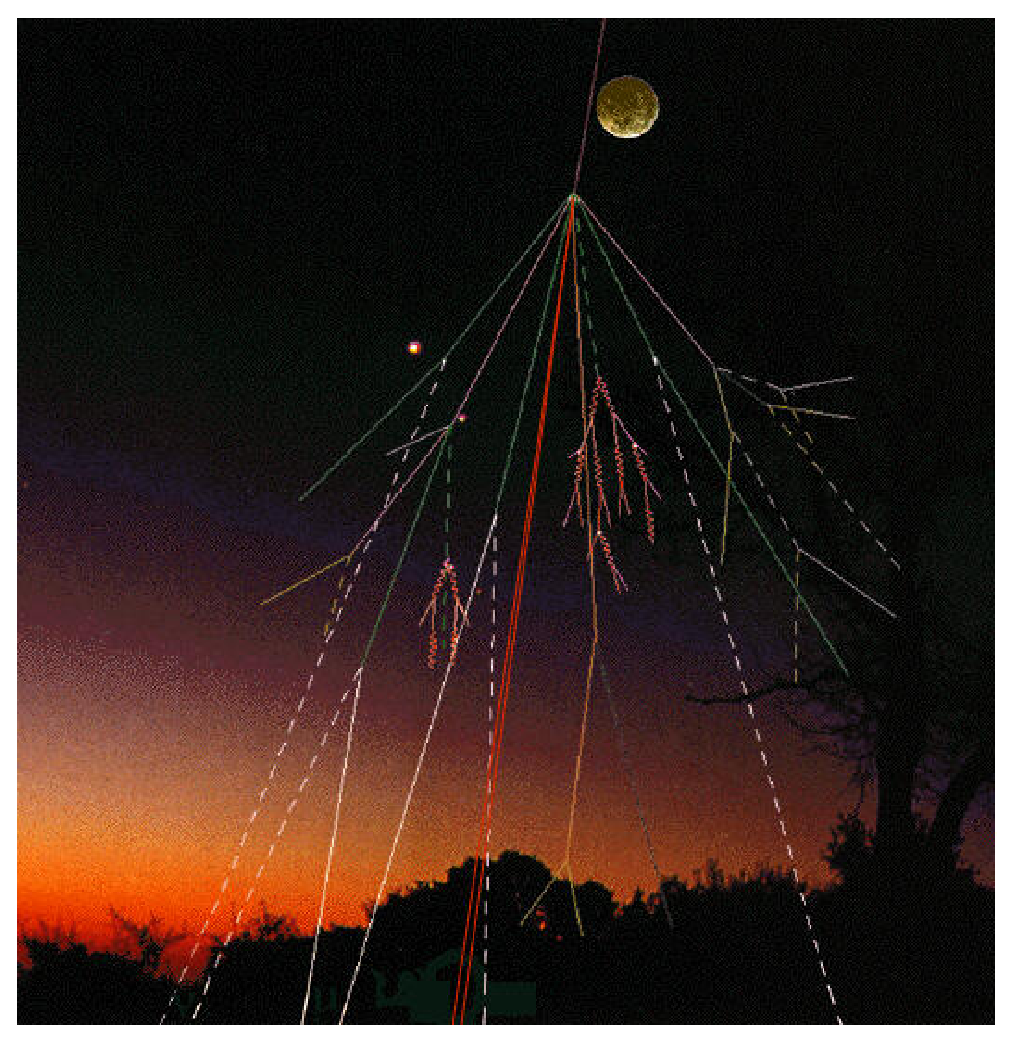
\includegraphics[scale=0.75]{shower}
\par\end{centering}

\caption{De intensiteit van de kosmische straling en ontstane deeltje in de
atmosfeer}
\end{figure}


Er zijn in deze grafiek drie gebieden te onderscheiden:

In gebied ``I'' ontstaan er steeds meer deeltjes door botsingen.
Het vervallen van deze deeltjes draagt nog nauwelijks bij tot het
aantal deeltjes.

In gebied ``II'' onstaan er globaal evenveel deeltjes als er vervallen.
De vervalproducten worden in de atmosfeer opgenomen en verdwijnen.

In gebied ``III'' neemt de dichtheid en daarmee de kans op botsingen
weer toe. Er ontstaan extra deeltjes die de absorbtie van de atmosfeer
ten dele compenseren.

We meten de hoeveelheid kosmische straling op de bodem. Er is dus
een hoogte in de atmosfeer waar meer kosmische straling wordt waargenomen.

\end{document}
